%\chapter{det-comp}


%%%%%%%%%%%%%%%%%%%%%%%%%%%%%%%%%%%%%%%%%%%%%%
%\section{Anode Plane Assemblies}

%%%%%%%%%%%%%%%%%%%%%%%%%%%%%%%%%%%%%%%%%%%%%%
\section{Cathode Plane Assembly (CPA)}
\label{sec:cpa}

%\subsection{Scope, requirements and design considerations}
\subsection{Scope and requirements}

The cathode plane, also called the cathode plane assembly, or CPA, is located in the middle of the TPC, dividing the detector into two equal-distance drift volumes. The cathode plane's 7\,m $\times$ 6\,m area is made up of six \textit{CPA columns}, each of which is constructed of three vertically stacked \textit{CPA modules}. The CPA therefore consists of 18 CPA modules. 

The scope of the CPA includes:

\begin{itemize}
\item 18 CPA modules, each with a frame and resistive cathode panel, 
\item HV bus connecting the CPA columns and modules, and
\item HV cup for receiving input from the power supply.
\end{itemize}


%%%%%%%%%%%%%%%%%%%%%%%%%
%\subsubsection{Requirements}
The CPA plane is required to:
\begin{itemize}
\item provide equipotential surfaces at $-$180kV nominal bias voltage,
\item maintain a flatness better than 1~cm when submerged in the liquid argon,
\item be constructed of materials with comparable CTEs to that of stainless steel, 
\item limit the electric field exposed to LAr to under 30~kV/cm 
\item prevent damage to the TPC, including its readout electronics, in case of a HV discharge anywhere on the cathode,
\item provide constant bias voltage and current to all attached field cage (FC) resistor divider chains,
\item support the full weight of the four connected top/bottom FC modules plus a person on the bottom FC during installation,
\item accommodate cryostat roof movement between warm and LAr-filled states,
\item be constructed in a modular form that can be easily installed in the cryostat,
\item accommodate Photon Detection System (PDS) calibration features, and
\item avoid any trapped volume of LAr.
\end{itemize}

%%%%%%%%%%%%%%%%%%%%%%%%%
\subsection{Design considerations}


For the future DUNE-SP far detector, the cathode planes are planned to be 12\,m tall by nearly 60\,m long.  When biased to the nominal voltage of $-$180\,kV, each of these cathode planes stores more than 100\,J of energy. If this energy were to be released  suddenly and completely in a high-voltage discharge event, it could greatly affect the integrity of the detector elements, including the sensitive front-end electronics.  
Study has shown~\cite{cathode-hv-1320} that a cathode plane made of interconnected metallic electrodes would present significant risk to the front-end ASICs based on the potential charge injection through the capacitive coupling between the cathode and the anode wires originating from such an event.  

To address this issue in ProtoDUNE, the entire cathode plane is made out of highly resistive material such that it has a very long discharge time constant.  In the event of HV breakdown at a given location on the cathode plane, the sudden change in voltage is restricted to  a relatively localized area on the CPA module in question.  The rest of the CPA maintains its original bias voltage, and gradually discharges to ground through the large resistivity of the cathode material.  This greatly reduces the instantaneous charge injection to the front-end electronics.


%%%%%%%%%%%%%%%%%%%%%%%%%
\subsection{CPA design}

%%%%%%%%%%%%%%%%%%%%%%%%%
\subsubsection{CPA modules}

%The cathode plane design has evolved through several iterations over the years.  The design chosen for the ProtoDUNE-SP TPC is an array of moderately sized modules constructed from strong FR4 (the fire-retardant version of G10) frames holding thin FR4 sheets laminated with a commercial resistive Kapton film on both sides.   Compared with the size of an APA, the CPA modules are 1/2 in width (1.16\,m) and 1/3 in height (2\,m).   Each module has four FR4 bars holding a 3mm thick FR4 sheet with resistive coating.  The thickness of the FR4 bars is 6cm.  The surfaces of the bars facing the APAs are covered by another set of resistive FR4 strip with a different bias voltage such that these FR4 bars do not cause any distortion in the drift field beyond the resistive surfaces.

The cathode plane design chosen for the ProtoDUNE-SP TPC is an array of 18 moderately sized modules constructed from strong 6-cm-thick FR4 (the fire-retardant version of G10) frames. The frames hold 3-mm-thick FR4 panels laminated on both sides with a commercial resistive Kapton film.   Each CPA module is 1.16\,m wide and 2\,m high, and they stack to form six CPA columns of height 6\,m.  The six-column-wide CPA has the same dimensions as each of the two APA planes, with a width of about 7\,m.

 The surface of the frame facing the APAs is covered by a set of resistive FR4 strips with a different bias voltage, set such that 
 the frame itself causes no distortion in the drift field beyond the resistive surfaces.

Each CPA column is suspended under the cathode support rail by a single insulating FR4 bar.  On the top and bottom edges of a CPA, two hinges support the partial weight of the top and bottom field cage modules.   Adjacent CPAs are aligned through pin-and-slot connections to maintain co-planarity while allowing minor relative vertical shifts due to cryostat roof movement.

The electrical connectivity of the resistive panels within a CPA column is maintained by several tabs through the edge frames.  There is no direct electrical connection across the CPA columns. 
Instead, the voltage is passed from one column to another through embedded cables in the CPA panels referred to collectively as the HV bus.  Redundant connections in the HV bus between CPA columns are used to ensure reliability.  
The HV bus also provides a low-resistance path for the voltage needed to operate the FC resistive divider chains.
The required connections to the FC modules are made at the edges of the cathode plane. 
Along the perimeter of the CPA, the HV bus cables are hidden between the field-shaping strip overhang and the main cathode resistive sheet.  The cables must be capable of withstanding the full cathode bias voltage to prevent direct arcing to (and as a result, the recharging of) a CPA panel that discharges to ground. 

The outer edges of the cathode plane facing the cryostat wall are populated with the same metal profiles, with insulating polyethylene caps, as used in the field cage.  This eliminates the need for a special design of the most crucial regions of the cathode plane: the edges of the CPA now look just like a continuation of the FC.  Since these profiles are the only objects facing grounded surfaces, they are the most likely candidates to have HV discharges to ground.   To limit peak current flow, these edge profiles are resistively connected to the field shaping strips.

%to the main cathode panels through
%their laminated resistive surfaces.  

The resistive surface concept is illustrated in Figure~\ref{fig:cpa-concept}.

\begin{cdrfigure}[Resistive surface CPA concept]{cpa-concept}{The resistive surface CPA concept showing  
 a 3D model of a corner of the cathode with major components.} 
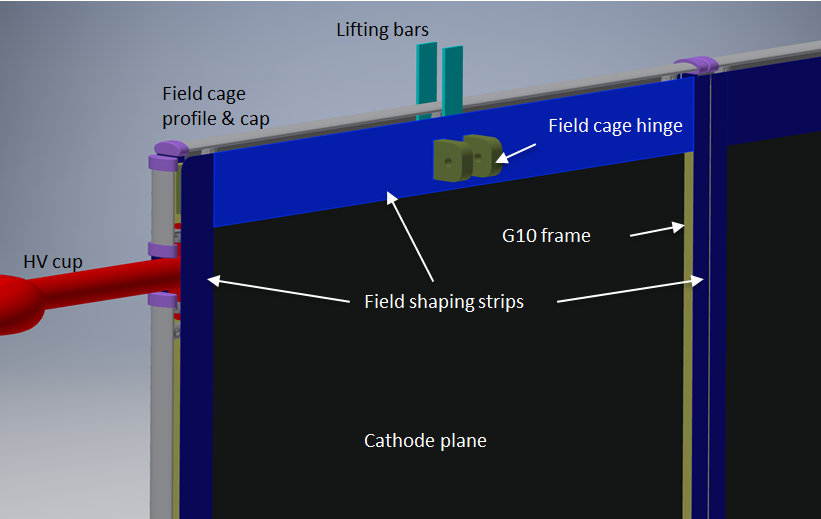
\includegraphics[width=\linewidth]{tpc_cpa_concept_leftonly}
\end{cdrfigure}


The CPA is connected to the HV feedthrough through a receptacle, called the \textit{HV cup}, at the back end of the cryostat (with respect to the beam entrance) and biased at $-$180\,kV.   It provides this voltage and the required current to all the FC modules (top, bottom and end walls) through electrical interconnects (Section~\ref{detcompsec-fc}). 

%The CPA is suspended by insulating bars from the CPA installation rail.  It also mechanically supports %six pairs of top/bottom FC modules.


%%%%%%%%%%%%%
%\subsubsection{Resistive material}

The main criteria for the selection of Kapton as the resistive material to be used to coat the CPA module panels are: %for the CPA modules are: 
\begin{itemize}
\item surface resistivity range,
\item compatibility with cryogenic temperatures,
\item robustness to HV discharges, 
\item material ageing,
\item radio-purity,
\item ability to coat a large surface area, and %availability on large area, and 
\item flatness, per the cathode flatness requirement. 
\end{itemize}

%The selected material is a \textregistered{Kapton} polyimide film made by \texttrademark{DuPont}.
%%%%%%%%%%%%
%\subsubsection{Support frame} % material properties}

Figures~\ref{fig:cpa-geometry} and~\ref{fig:cpa-view2} show the basic geometry of the cathode plane. Figure~\ref{fig:cpa-view2}a shows the block at the top of a CPA that is secured to the top cross bar and extends to the top supporting I-beam.  This block must support the weight of four half FCs (4 $\times$ 150~lbs) and the weight of the CPA itself (160~lbs) for a total weight of approximately 750~lbs.  Design analysis was done with earlier, heavier FCs (220~lbs). Figure~\ref{fig:cpa-hinge1} shows how the FC is attached to the assembled cathode plane. 

\begin{cdrfigure}[CPA geometry]{cpa-geometry}{Basic geometry of the CPA array, close ups and a CPA column (on its side)} 
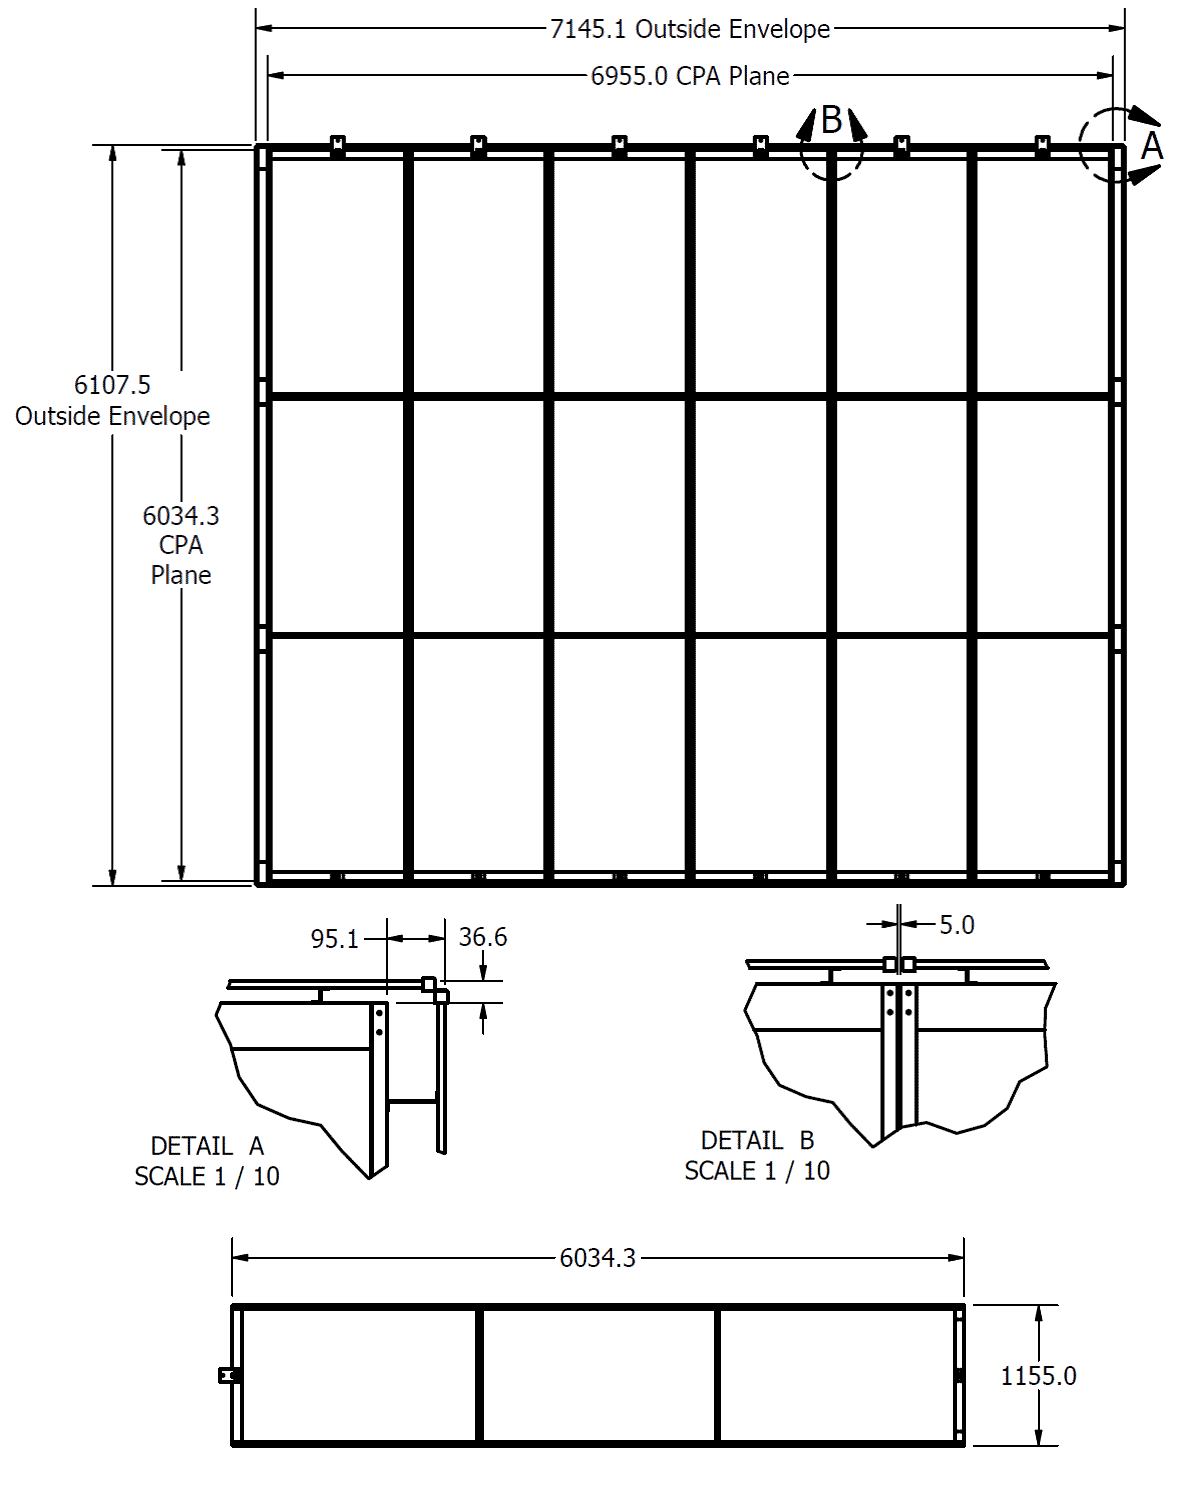
\includegraphics[width=\linewidth]{tpc_cpa_front_views1}
\end{cdrfigure}

\begin{cdrfigure}[Views of various parts of a CPA]{cpa-view2}{Views of various parts of a CPA. Top: the block at the top of a CPA. Middle: hardware connecting two vertically stacked CPA modules. Bottom: connection between two adjacent CPA columns.} 
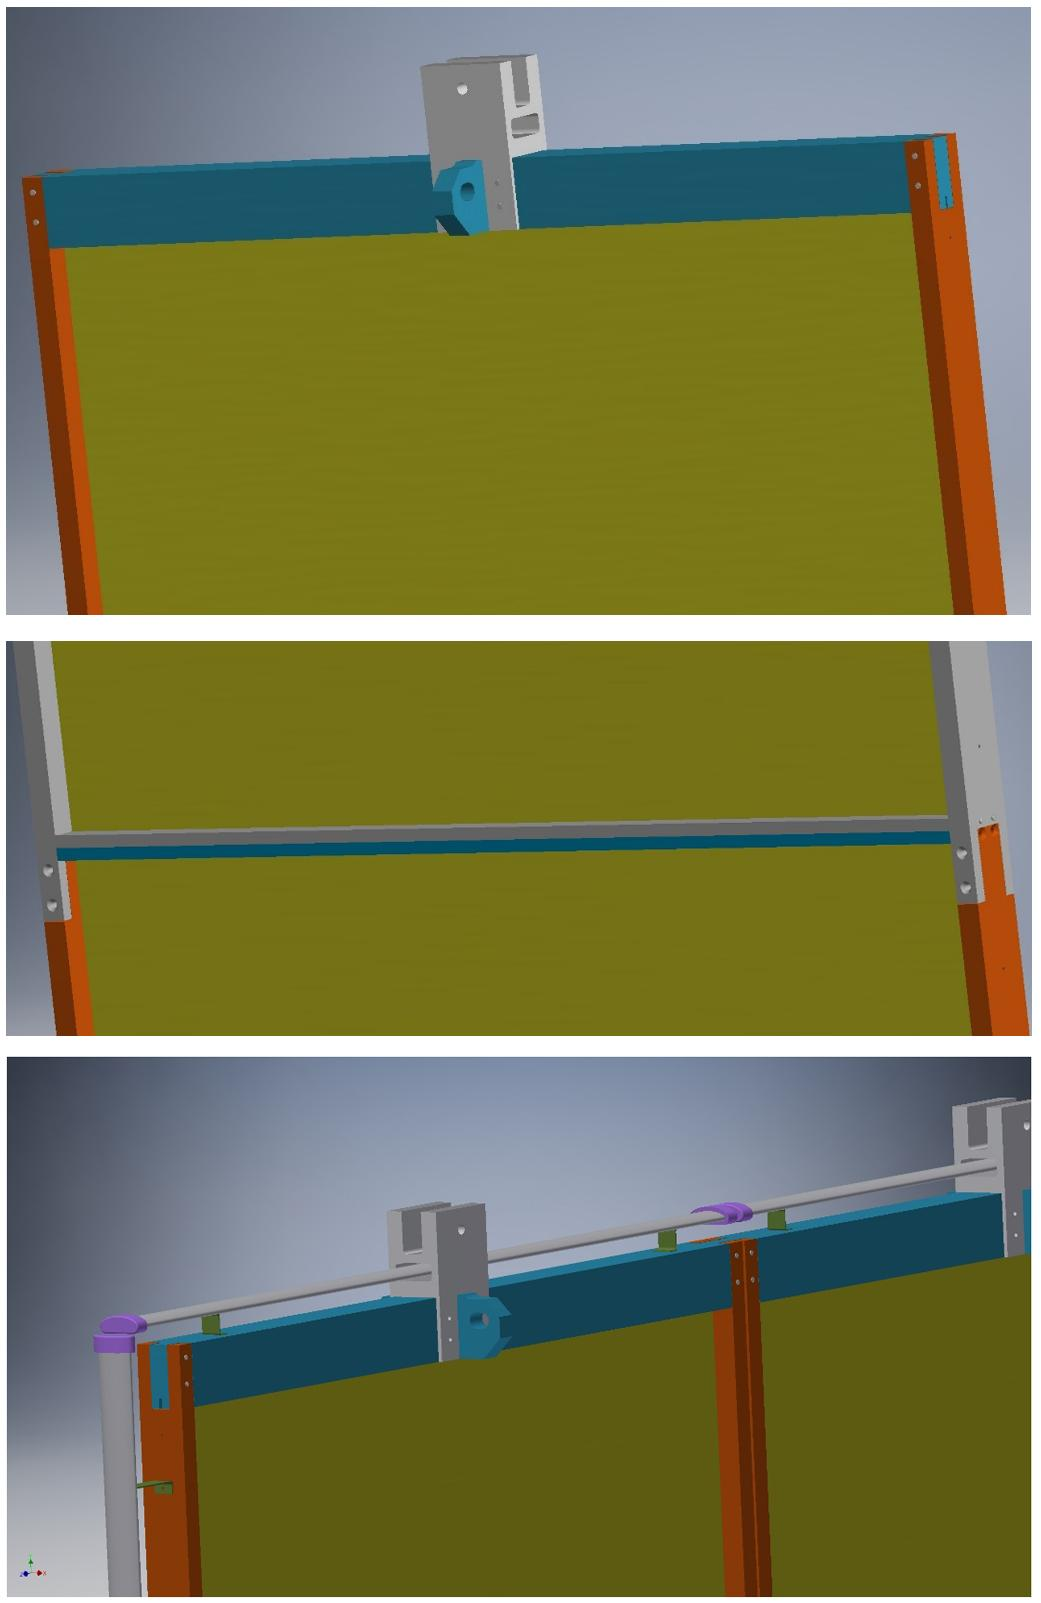
\includegraphics[width=0.8\linewidth]{tpc_cpa_views2}
\end{cdrfigure}

\begin{cdrfigure}[Hinged connection between CPA and FC module]{cpa-hinge1}{Hinged connection between CPA and FC module; the top field cage modules are hung vertically with the CPAs when moved into the cryostat, then rotated to horizontal to attach to the APA.} 
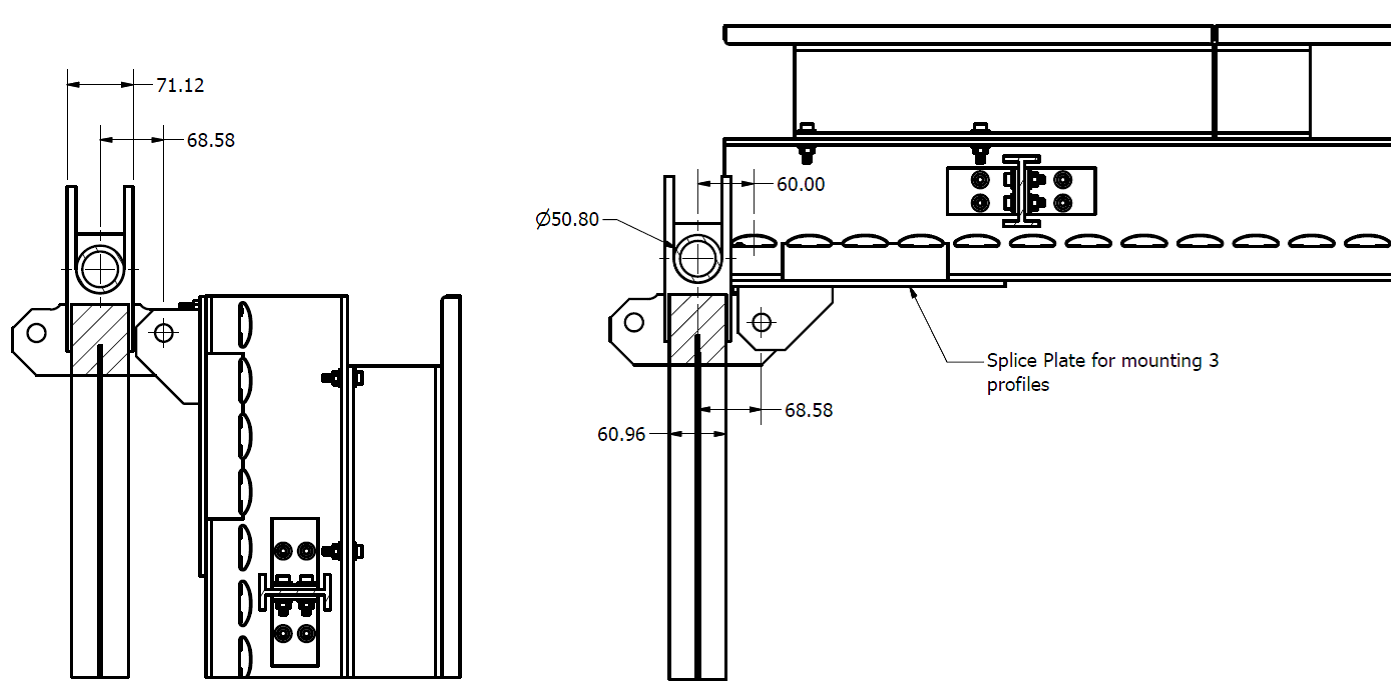
\includegraphics[width=\linewidth]{tpc_cpa_fc_hinge}
\end{cdrfigure}


\textit{Deformation and stress due to pressure from circulating LAr}

Calculations indicate that a uniform 2-Pa pressure 
  applied to the resistive panels  during cooldown will result in 0.090~inch deflections of the panel at its center.  The entire TPC (i.e., the CPA/FC/APA assembly) will displace 8.8~mm laterally as a result of the net force from this pressure.  

\textit{Thermal considerations}

When the CPA modules are cooled, their width will shrink by 0.9~mm.  The supporting stainless steel beam will shrink by 1.6~mm over the width of the CPA.  If the CPA supports are rigidly attached to the supporting stainless steel beam, then an interference of 0.7~mm (the difference) will occur.  To prevent this interference and ensure contact between CPAs after cooldown, an initial gap of 0.7~mm between CPAs is required.  

The steel beam between the CPA and APA will shrink by 5.2~mm relative to the field cage length when cooled to LAr temperature.  The joint between the FC and the CPA is designed to accommodate this shrinkage.



%%%%%%%%%%%%
\subsection{Mechanical and electrical interconnections between modules}

Three modules are stacked vertically to form the 6-m height of a CPA. %the ProtoDUNE-SP  cathode.  
The frames of these modules are bolted together using tongue-and-groove connections at the ends. The resistive cathode sheets and the field-shaping strips are connected using metallic tabs to ensure redundant electrical contact between the CPAs. %vertical modules. 


%There are six 6\,m tall CPA modules in  ProtoDUNE-SP.  
Each CPA is suspended from the cathode rail using a central lifting bar.  Due to the roof movement between the warm and cold phases of the cryostat as it is cooled, each CPA is expected to move $\sim$2~mm relative to its neighbors.  Several pin-and-slot connections are implemented at the long edges of the CPA columns to ensure the co-planarity of the modules while allowing for a small vertical displacement.  

The HV bus provides the high voltage to the FC
circuits and CPA modules with a voltage drop much less than 0.1\% of the
default voltage. The location of the bus with respect to the CPA frame is shown in Figure~\ref{fig:HVbusmodel}. The field-shaping electrodes on the faces of the CPA module
frames are part of the FC circuit, described in Section~\ref{detcompsec-fc}. 
FC electrodes on the outer edges of the
CPA are held at the cathode potential to provide field
uniformity and to protect the HV bus from discharge.  

\begin{cdrfigure}[Model of the HV bus]{HVbusmodel}{A perspective view of CPA frame showing the location of the HV bus cable and attachments to the HV cup and resistive cathode, with CPA frame electrodes omitted to make HV bus visible.}
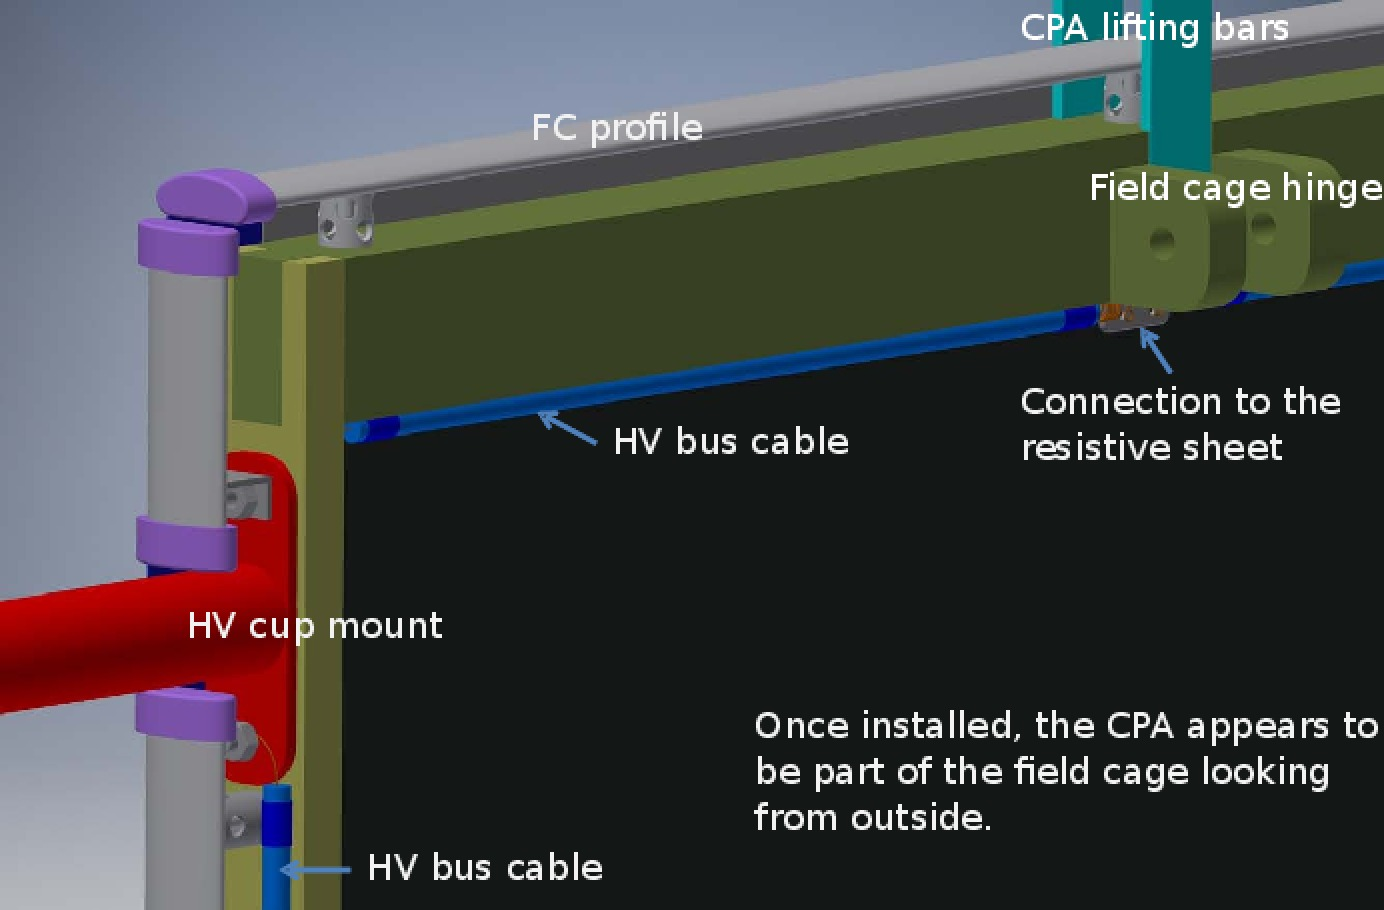
\includegraphics[height=0.35\textheight]{DUNE_SP_CPA_Design_Update-slide17-mod}
\end{cdrfigure}


